%%%%%%%%%%%%%%%%%%%%%%%%%%%%%%%%%%%%%%%%%
% Short Sectioned Assignment
% LaTeX Template
% Version 1.0 (5/5/12)
%
% This template has been downloaded from:
% http://www.LaTeXTemplates.com
%
% Original author:
% Frits Wenneker (http://www.howtotex.com)
%
% License:
% CC BY-NC-SA 3.0 (http://creativecommons.org/licenses/by-nc-sa/3.0/)
%
%%%%%%%%%%%%%%%%%%%%%%%%%%%%%%%%%%%%%%%%%

%----------------------------------------------------------------------------------------
%   PACKAGES AND OTHER DOCUMENT CONFIGURATIONS
%----------------------------------------------------------------------------------------

\documentclass[11pt, oneside]{article} % A4 paper and 11pt font size
\usepackage[margin=1in]{geometry}
\geometry{letterpaper}

\usepackage{pslatex}
\usepackage[T1]{fontenc} % Use 8-bit encoding that has 256 glyphs
\usepackage[english]{babel} % English language/hyphenation
\usepackage{amsmath,amsfonts,amsthm} % Math packages

\usepackage{lipsum} % Used for inserting dummy 'Lorem ipsum' text into the template

\usepackage{graphicx} % Required for including pictures
\usepackage{wrapfig}
\usepackage{caption}
\usepackage{subcaption}
\usepackage{float}
\usepackage{enumitem}
\usepackage{listings}
\usepackage{color}
\usepackage[]{hyperref}


\usepackage{sectsty} % Allows customizing section commands

\numberwithin{equation}{section} % Number equations within sections (i.e. 1.1, 1.2, 2.1, 2.2 instead of 1, 2, 3, 4)
\numberwithin{figure}{section} % Number figures within sections (i.e. 1.1, 1.2, 2.1, 2.2 instead of 1, 2, 3, 4)
\numberwithin{table}{section} % Number tables within sections (i.e. 1.1, 1.2, 2.1, 2.2 instead of 1, 2, 3, 4)

%\setlength\parindent{0pt} % Removes all indentation from paragraphs - comment this line for an assignment with lots of text

\newcommand{\code}[1]{\texttt{#1}}
\newcommand\todo[1]{\textbf{\textcolor{red}{#1}}}

%----------------------------------------------------------------------------------------
%   TITLE SECTION
%----------------------------------------------------------------------------------------

\title{ 
Tweetnet: Looking for Botnets on Twitter\
}

\author{
Josh Blum (blum)\\
Bennet Cyphers (benny)\\
Ofir Nachum (ofir)\\
Louis Sobel (sobel)\\
\\
6.857 Final Project
\date{\today}
}

\begin{document}

\maketitle

\vfill

\begin{abstract}
\todo{blah blah black sheep}
\end{abstract}

\clearpage

\section {Introduction}

\section {Related Work}
Botnets using social networks for command and control are a relatively recent phenomenon.  These botnets take advantage of the reliable infrastructure and easy-to-use APIs of social networks to communicate commands to infected computers.  Several of these botnets have already been detected.  

Several botnets have been discovered in the wild \cite{arbor, trendmicro, flashback}.  In 2009, Arbor Networks \cite{arbor} discovered a Twitter bot which periodically tweets base-64 encoded commands that specify URLs for downloading malicious binaries.  The Mehika botnet \cite{trendmicro} is another botnet which was found utilizing Twitter to send commands to its botslaves.  The Macintosh Flashware malware provides another example of a botnet using Twitter for command and control \cite{flashback}.  The malware queries Twitter for tweets containing specific hashtags.  

In addition to these detected botnets, several groups have designed and implemented social networking botnets \cite{socialnetworking, trojan7, stegobot}.  A group of San Jose University researchers design and implement their \emph{SocialNetworkingBot} to issue commands via Twitter for such things as browsing a URL, taking a screenshot, shutting down the computer, or changing botmaster \cite{socialnetworking}.  Another notable example is a group of researches developing \emph{Stegobot}, a botnet which covertly communicates via JPEG stegonography of images shared on social networks.  These examples highlight the ease in which it is possible to use social networks as botnet infrastructure.

In response the the growing threat of botnets using social networks, researchers have proposed several detection mechanisms to thwart such botnets \cite{botsniffer, kartaltepe, burghouwt}.  Gu et al. propose an approach using network-based anomaly detection \cite{botsniffer}.  These methods are useful when botnet activity is temporally correlated.  Kartaltepe et al. present a content-specific method, proposing a classifier for classifying natural text from base-64 or otherwise encoded commands \cite{kartaltepe}.  The group also suggests client-side detection mechanisms that are alerted by network traffic of dubious origin (for example, if a Twitter URL is requested when no browser actually has Twitter displayed).

The previous work in this field shows that, while botnets using social networks is a relatively recent phenomenon, the threat of even better concealed botnets is growing rapidly.  For this reason, it is imperative that new detection mechanisms be devised.

\section{Game Overview}
	\subsection{Justification}
	\subsection{Infrastructure}
	\subsection{Rules}

\section{Meet the Team}
	\subsection{Team Blumbenny}

	\begin{figure}
		\centering
		\begin{subfigure}{.4\textwidth}
			\centering
			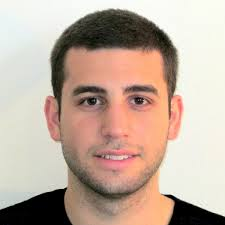
\includegraphics[width=.4\textwidth]{resources/blum.jpg}
			\caption{Blum}
		\end{subfigure}
		\begin{subfigure}{.4\textwidth}
			\centering
			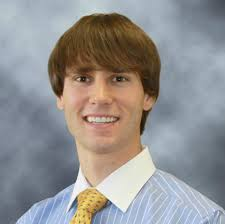
\includegraphics[width=.4\textwidth]{resources/benny.jpg}
			\caption{Benny}
		\end{subfigure}
		\caption{Team Blumbenny}
	\end{figure}


	\subsection{Team Lofir}
	
		\begin{figure}
		\centering
		\begin{subfigure}{.4\textwidth}
			\centering
			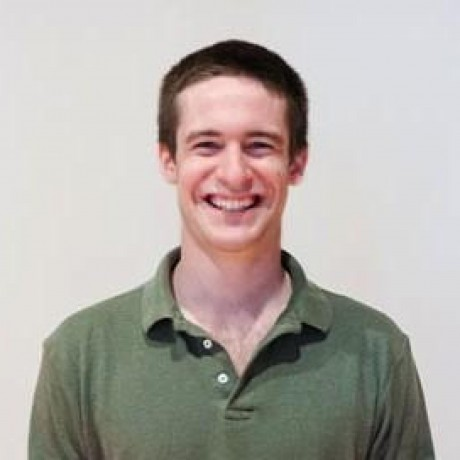
\includegraphics[width=.4\textwidth]{resources/louis.jpg}
			\caption{Louis}
		\end{subfigure}
		\begin{subfigure}{.4\textwidth}
			\centering
			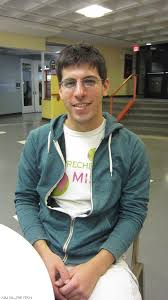
\includegraphics[width=.4\textwidth]{resources/ofir.jpg}
			\caption{Ofir}
		\end{subfigure}
		\caption{Team Lofir}
	\end{figure}

\section{Round 1}
	\subsection{Setup}
	\subsection{Designs}
	\subsection{Attacks}
	\subsection{Problems}

\section{Round 2}
	\subsection{Modifications}
	\subsection{Designs}
	\subsection{Attacks}
	\subsection{Problems}

\section{Discussion}

	\subsection{What we learned}
	\subsection{How this extends to real twitter}
	\subsection{How this does \textit{not} extend to real twitter}
	\subsection{Future Designs / work}

\section{Conclusion}


\clearpage
\section{References}

\begingroup
\renewcommand{\section}[2]{}%
\begin{thebibliography}{99}

\bibitem{arbor}
	\url{http://www.arbornetworks.com/asert/2009/08/twitter-based-botnet-command-channel/}

\bibitem{trendmicro}
	\url{http://www.trendmicro.com/cloud-content/us/pdfs/security-intelligence/white-papers/wp_discerning-relationships__mexican-botnet.pdf}

\bibitem{cryptome}
	\url{http://cryptome.org/2014/03/massive-twitter-botnet.htm}

\bibitem{socialnetworking}
	\url{http://www.mecs-press.org/ijcnis/ijcnis-v5-n6/IJCNIS-V5-N6-2.pdf}

\bibitem{trojan7}
	\url{http://trojan7malware.blogspot.com/2013/06/botnet-using-twitter-as-c.html}

\bibitem{flashback}
	\url{http://www.intego.com/mac-security-blog/flashback-mac-malware\%2Duses-twitter-as-command-and-control-center/}

\bibitem{botsniffer}
	\url{http://corescholar.libraries.wright.edu/cgi/viewcontent.cgi?article=1006&context=cse}

\bibitem{kartaltepe}
	\url{http://link.springer.com/chapter/10.1007/978-3-642-13708-2_30}

\bibitem{burghouwt}
	\url{http://link.springer.com/chapter/10.1007/978-3-642-25560-1_9}

\bibitem{botnet_survey}
	\url{http://www.sciencedirect.com/science/article/pii/S1389128612003568#}

\bibitem{stegobot}
	\url{http://www.cs.utexas.edu/~amir/papers/IH11-Stegobot.pdf}

\bibitem{skype}
	\url{http://link.springer.com/chapter/10.1007\%2F978-3-642-14215-4_5}

\end{thebibliography}

\endgroup

\end{document}



